% Copyright © 2012-2013 Martin Ueding <dev@martin-ueding.de>
%
% Copyright © 2012 Martin Ueding <dev@martin-ueding.de>
%
\documentclass[11pt, ngerman, fleqn]{scrartcl}

\usepackage{graphicx}

%%%%%%%%%%%%%%%%%%%%%%%%%%%%%%%%%%%%%%%%%%%%%%%%%%%%%%%%%%%%%%%%%%%%%%%%%%%%%%%
%                                Locale, date                                 %
%%%%%%%%%%%%%%%%%%%%%%%%%%%%%%%%%%%%%%%%%%%%%%%%%%%%%%%%%%%%%%%%%%%%%%%%%%%%%%%

\usepackage{babel}
\usepackage[iso]{isodate}

%%%%%%%%%%%%%%%%%%%%%%%%%%%%%%%%%%%%%%%%%%%%%%%%%%%%%%%%%%%%%%%%%%%%%%%%%%%%%%%
%                          Margins and other spacing                          %
%%%%%%%%%%%%%%%%%%%%%%%%%%%%%%%%%%%%%%%%%%%%%%%%%%%%%%%%%%%%%%%%%%%%%%%%%%%%%%%

\usepackage[activate]{pdfcprot}
\usepackage[left=3cm, right=2cm, top=2cm, bottom=2cm]{geometry}
\usepackage[parfill]{parskip}
\usepackage{setspace}

\setlength{\columnsep}{2cm}

%%%%%%%%%%%%%%%%%%%%%%%%%%%%%%%%%%%%%%%%%%%%%%%%%%%%%%%%%%%%%%%%%%%%%%%%%%%%%%%
%                                    Color                                    %
%%%%%%%%%%%%%%%%%%%%%%%%%%%%%%%%%%%%%%%%%%%%%%%%%%%%%%%%%%%%%%%%%%%%%%%%%%%%%%%

\usepackage{color}

\definecolor{darkblue}{rgb}{0,0,.5}
\definecolor{darkgreen}{rgb}{0,.5,0}
\definecolor{darkred}{rgb}{.7,0,0}

%%%%%%%%%%%%%%%%%%%%%%%%%%%%%%%%%%%%%%%%%%%%%%%%%%%%%%%%%%%%%%%%%%%%%%%%%%%%%%%
%                         Font and font like settings                         %
%%%%%%%%%%%%%%%%%%%%%%%%%%%%%%%%%%%%%%%%%%%%%%%%%%%%%%%%%%%%%%%%%%%%%%%%%%%%%%%

\usepackage[charter, greekuppercase=italicized]{mathdesign}
\usepackage{beramono}
\usepackage{berasans}

% Style of vectors and tensors.
\newcommand{\tens}[1]{\boldsymbol{\mathsf{#1}}}
\renewcommand{\vec}[1]{\boldsymbol{#1}}

%%%%%%%%%%%%%%%%%%%%%%%%%%%%%%%%%%%%%%%%%%%%%%%%%%%%%%%%%%%%%%%%%%%%%%%%%%%%%%%
%                               Input encoding                                %
%%%%%%%%%%%%%%%%%%%%%%%%%%%%%%%%%%%%%%%%%%%%%%%%%%%%%%%%%%%%%%%%%%%%%%%%%%%%%%%

\usepackage[T1]{fontenc}
\usepackage[utf8]{inputenc}

%%%%%%%%%%%%%%%%%%%%%%%%%%%%%%%%%%%%%%%%%%%%%%%%%%%%%%%%%%%%%%%%%%%%%%%%%%%%%%%
%                         Hyperrefs and PDF metadata                          %
%%%%%%%%%%%%%%%%%%%%%%%%%%%%%%%%%%%%%%%%%%%%%%%%%%%%%%%%%%%%%%%%%%%%%%%%%%%%%%%

\usepackage{hyperref}
\usepackage{lastpage}

\hypersetup{
	breaklinks=false,
	citecolor=darkgreen,
	colorlinks=true,
	linkcolor=black,
	menucolor=black,
	pdfauthor={Martin Ueding},
	urlcolor=darkblue,
}

%%%%%%%%%%%%%%%%%%%%%%%%%%%%%%%%%%%%%%%%%%%%%%%%%%%%%%%%%%%%%%%%%%%%%%%%%%%%%%%
%                               Math Operators                                %
%%%%%%%%%%%%%%%%%%%%%%%%%%%%%%%%%%%%%%%%%%%%%%%%%%%%%%%%%%%%%%%%%%%%%%%%%%%%%%%

\usepackage[thinspace, squaren]{SIunits}
\usepackage{amsmath}
\usepackage{amsthm}
\usepackage{commath}

% Word like operators.
\DeclareMathOperator{\acosh}{arcosh}
\DeclareMathOperator{\arcosh}{arcosh}
\DeclareMathOperator{\arcsinh}{arsinh}
\DeclareMathOperator{\arsinh}{arsinh}
\DeclareMathOperator{\asinh}{arsinh}
\DeclareMathOperator{\card}{card}
\DeclareMathOperator{\diam}{diam}
\renewcommand{\Im}{\mathop{{}\mathrm{Im}}\nolimits}
\renewcommand{\Re}{\mathop{{}\mathrm{Re}}\nolimits}

% Special single letters.
\DeclareMathOperator{\fourier}{\mathcal{F}}
\newcommand{\C}{\ensuremath{\mathbb C}}
\newcommand{\ee}{\mathrm e}
\newcommand{\ii}{\mathrm i}
\newcommand{\N}{\ensuremath{\mathbb N}}
\newcommand{\R}{\ensuremath{\mathbb R}}
\newcommand{\Z}{\ensuremath{\mathbb Z}}

% Shape like operators.
\DeclareMathOperator{\dalambert}{\Box}
\DeclareMathOperator{\laplace}{\bigtriangleup}
\newcommand{\curl}{\vnabla \times}
\newcommand{\divergence}[1]{\inner{\vnabla}{#1}}
\newcommand{\vnabla}{\vec \nabla}

% Shortcuts
\newcommand{\ev}{\hat{\vec e}}
\newcommand{\e}[1]{\cdot 10^{#1}}
\newcommand{\half}{\frac 12}
\newcommand{\inner}[2]{\left\langle #1, #2 \right\rangle}

% Placeholders.
\newcommand{\emesswert}{\del{\messwert \pm \messwert}}
\newcommand{\fehlt}{\textcolor{darkred}{Hier fehlen noch Inhalte.}\marginpar{\textcolor{darkred}{!}}}
\newcommand{\messwert}{\textcolor{blue}{\square}}
\newcommand{\punkte}{\textcolor{white}{xxxxx}}

%%%%%%%%%%%%%%%%%%%%%%%%%%%%%%%%%%%%%%%%%%%%%%%%%%%%%%%%%%%%%%%%%%%%%%%%%%%%%%%
%                                  Headings                                   %
%%%%%%%%%%%%%%%%%%%%%%%%%%%%%%%%%%%%%%%%%%%%%%%%%%%%%%%%%%%%%%%%%%%%%%%%%%%%%%%

\usepackage{scrpage2}

\pagestyle{scrheadings}

\automark{section}
\cfoot{\footnotesize{Seite \thepage\ / \pageref{LastPage}}}
\chead{}
\ihead{}
\ohead{\rightmark}
\setheadsepline{.4pt}


\usepackage{tikz}

\newcommand{\themodul}{physik321}
\newcommand{\thegruppe}{Gruppe 8 -- Julia Volmer}
\newcommand{\theuebung}{11}

\ifoot{\footnotesize{Martin Ueding, Simon Schlepphorst}}
\ihead{\themodul{} -- Übung \theuebung}
\ofoot{\footnotesize{\thegruppe}}

\def\thesection{H \theuebung.\arabic{section}}
\def\thesubsubsection{\thesubsection\alph{section}}

\title{\themodul{} -- Übung \theuebung \\ \vspace{0.5cm} \large{\thegruppe}}

\author{
	Martin Ueding \\ \small{\href{mailto:mu@uni-bonn.de}{mu@uni-bonn.de}}
	\and
	Simon Schlepphorst \\ \small{\href{mailto:s2@uni-bonn.de}{s2@uni-bonn.de}}
}

\hypersetup{
	pdftitle={\themodul {} - Übung \theuebung},
}

\begin{document}

\maketitle

\begin{table}[h]
	\centering
	\begin{tabular}{l|c|c|c|c}
		Aufgabe
		& \ref 1
		& \ref 2
		& \ref 3
		& $\sum$   \\
		\hline
		Punkte
		& \punkte / 20
		& \punkte / 10
		& \punkte / 20
		& \punkte / 50
	\end{tabular}
\end{table}

%%%%%%%%%%%%%%%%%%%%%%%%%%%%%%%%%%%%%%%%%%%%%%%%%%%%%%%%%%%%%%%%%%%%%%%%%%%%%%%
%                              Die Lorentzgruppe                              %
%%%%%%%%%%%%%%%%%%%%%%%%%%%%%%%%%%%%%%%%%%%%%%%%%%%%%%%%%%%%%%%%%%%%%%%%%%%%%%%

\section{Die Lorentzgruppe}
\label 1

\subsection{Motivation der Einteilung}

Die Länge $d := \norm{\vec x} = \sqrt{\inner{\vec x}{\vec x}} = \sqrt{\vec x
\tens g \vec x} = \sqrt{x^\mu x^\nu g_{\mu \nu}}$ ist physikalisch die
Eigenzeit. Für eine Reise entlang des Vektors $\vec x$ vergeht diese Eigenzeit.
Reisen innerhalb des Lichtkegels erfordern eine positive Zeit, entlang des
Kegels sind Lichtstrahlen, für die keine Eigenzeit vergeht. Reisen entlang
Vektoren $\vec x$, die nicht innerhalb des Kegels liegen, sind nicht möglich,
daher eine imaginäre Reisezeit.

Somit können wir Reisen mit $d = 0$ als lichtartig bezeichnen. Entfernungen,
die innerhalb des Kegels liegen, haben ihre Hauptentfernung (Maximumsnorm) in
der Zeit und können so als zeitartig bezeichnet werden. Entfernungen zwischen
zwei Ereignissen, die gleichzeitig (geht nur bezüglich des aktuellen Systems)
passieren, ist sinnvollerweise raumartig. Ihr Abstandsquadrat $d^2$ ist kleiner
als null, so dass dies passt.

\subsection{nur lineare Abbildungen}

Nur lineare Abbildungen lassen die physikalisch sinnvolle Größe, die Eigenzeit
$d$, invariant. Dies lässt sich am einfachsten in der Penrose-Notation
darstellen. \cite{penrose-road_to_reality}

Dazu definieren wir folgende Symbole gemäß der Notation. Dabei sind Tensoren
die geometrischen Formen, Indizes nach oben (Vektor) und unten (Kovektor)
werden durch Anfasser oben beziehungsweise unten dargestellt. Der metrische
Tensor ist einfach ein Bügel:
\begin{center}
	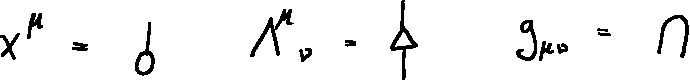
\includegraphics{H1-Definitionen.pdf}
\end{center}

Kontraktion wird in dieser Notation über das Verbinden von Indizes dargestellt.
So ist das Skalarprodukt:
\begin{center}
	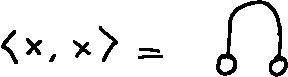
\includegraphics{H1-Skalarprodukt.pdf}
\end{center}

Nun wenden wir die Transformation $\tens \Lambda$ an, kontrahieren $\vec x$
also mit $\tens \Lambda$:
\begin{center}
	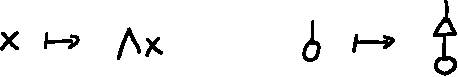
\includegraphics{H1-Transformation.pdf}
\end{center}

Das Skalarprodukt wird auch transformiert. Wir fügen noch zwei metrische
Tensoren ein und benutzen die Umkehrabbildung $\tens \Lambda^{-1}$. Da die
Transformation aus der Symmetriegruppe des Minkoswkiraums, $O(1, 3)$ stammt,
ist die Transformationsmatrix $\tens \Lambda$ es eine orthonormale Matrix.
Daher ist die inverse Matrix nur die Transponierte. Diese erhalten wir, wie in
der nächsten Zeichnung schon enthalten, über Kontraktion mit zwei metrischen
Tensoren ($\Lambda^\alpha{}_\beta \mapsto \Lambda_\gamma{}^\eta$). Wäre $\tens
\Lambda$ keine lineare Abbildung, sondern etwas allgemeineres, gäbe es zum
einen keine Komponentendarstellung, zum anderen wäre das Inverse nicht das
Transponierte.

Im nächsten
Schritt nutzen wir auch aus, dass $g_{\mu\nu} g^{\nu\xi} = \delta_\mu{}^\xi$.
Dann nutzen wir aus, dass $\tens \Lambda \tens \Lambda^{-1} = \tens 1$. Wir
erhalten das ursprüngliche Skalarprodukt:
\begin{center}
	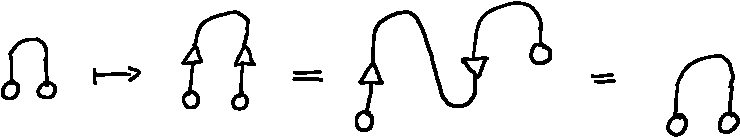
\includegraphics{H1-Invarianz.pdf}
\end{center}

Das ganze können wir auch noch rechnerisch zeigen:
\begin{align*}
	\inner{\vec x}{\vec x}
	&= x^\alpha g_{\alpha \beta} x^\beta \\
	\intertext{Wir bilden mit $\tens \Lambda$ ab.}
	&\mapsto \Lambda^\gamma{}_\alpha x^\alpha g_{\gamma \eta}
	\Lambda^\eta{}_\beta x^\beta \\
	\intertext{%
		Wir führen zwei weitere metrische Tensoren ein und benutzen die
		Umkehrabbildung $\tens \Lambda^{-1} =: \tilde{\tens \Lambda}$.
	}
	&= \Lambda^\gamma{}_\alpha x^\alpha g_{\gamma \xi} g^{\xi \eta}
	\tilde\Lambda_\eta{}^\iota g_{\iota\beta} x^\beta \\
	\intertext{%
		Die beiden metrischen Tensoren werden zu einem $\delta$ wegen
		$g_{\mu\nu} g^{\nu\xi} = \delta_\mu{}^\xi$, so dass sich die Indizes
		$\gamma$ und $\eta$ identisch werden.
	}
	&= \Lambda^\gamma{}_\alpha x^\alpha \tilde\Lambda_\gamma{}^\iota
	g_{\iota\beta} x^\beta \\
	\intertext{%
		Wir nutzen aus, dass $\tens \Lambda \tens \Lambda^{-1} = \tens 1$.
	}
	&= \delta^\iota{}_\alpha x^\alpha g_{\iota\beta} x^\beta \\
	\intertext{%
		Wir führen noch das letzte $\delta$ aus und erhalten unsere
		ursprüngliche Summe:
	}
	&= x^\alpha g_{\alpha\beta} x^\beta \\
	&= \inner{\vec x}{\vec x}
\end{align*}

\subsection{Forderung nach Konstanz der Lichtgeschwindigkeit}

Bei einer Lorentztransformation $\tens \Lambda$ soll die Lichtgeschwindigkeit
konstant bleiben. Unter anderem wollen wir, dass lichtartige Wege (ohne
Eigenzeit) weiterhin ohne Eigenzeit sind. Dies ist formal:
\[
	\norm{\vec x} = 0 \implies \norm{\tens \Lambda \vec x} = 0
\]

Wir haben in der vorherigen Aufgabe schon gezeigt, dass die
Lorentztransformation das Skalarprodukt überhaupt nicht ändert. Von daher
können wir sicher einen Faktor $a(\tens \Lambda) = 1$ einfügen.

\subsection{Faktor gleich eins}

Siehe oben.

\subsection{Isometriebedingung}

Das ist letztlich das, was wir weiter oben schon benutzt haben. Unsere
Herleitung hat ja gerade nur deshalb funktioniert, weil das Inverse das
Transponierte ist. Von daher haben wir die Isometriebedingung schon gefolgert.

\subsection{räumliche Drehungen als Lorentztransformation}

Die Symmetriegruppe des Minkoswkiraums $\mathbb M$ ist $O(1, 3)$. Lassen wir
die Zeit weg, erhalten wir den normalen, drei dimensionalen, Euklidischen Raum
$\mathbb E^3$. Die Symmetriegruppe ist dort $O(3)$.

\subsection{Zeitumkehr und Parität}

$\tens T$ und $\tens P$ sind orthonormale Matrizen. Dies ist schnell daran zu
sehen, dass das Inverse das Transponierte ist. Da beide Transformationen
Umkehrungen sind, ist die gleiche Transformation auch die Umkehrtransformation.
Somit gilt sogar:
\[
	\tens T = \tens T^T = \tens T^{-1}
\]
Analog für $\tens P$.

\subsection{Zeitdilatation und Determinante}

$\Lambda^0{}_0$ ist ein Zeitstreckungsfaktor. Dieser muss betragsmäßig größer
als eins sein.

Die Determinante einer orthonormalen Matrix aus $SO(3)$ und $SO(1, 3)$ muss 1
sein. Da wir auch Abbildungen zulassen, die die Orientierung umkehren, also aus
$O(1, 3)$, darf auch $-1$ heraus kommen.

\subsection{negativer Zeitstreckungsfaktor}

Bei negativem Zeitstreckungsfaktor wird die Zeit umgekehrt. Es ist also eine
Transformation aus $SO(1, 3)$ zusammen mit der Zeitumkehr.

\subsection{Gruppe}

Wir müssen die Gruppenaxiome nachrechnen. Da wir die Elemente der Gruppe als
Matrizen darstellen können, können wir einiges überspringen.

Die Gruppe ist bezüglich folgender Verknüpfung $\circ$ gemeint:
\[
	\tens B \circ \tens A = \tens B \tens A
	\iff
	\del{\tens B \circ \tens A}^\alpha{}_\beta
	= B^\alpha{}_\gamma A^\gamma{}_\beta
\]

\begin{description}
	\item[neutrales Element]
		Als neutrales Element erfüllt die Einheitsmatrix die
		Neutralitätsbedingung: $\tens 1 \circ \tens A = \tens A$.

	\item[Assoziativität]
		Da Matrizen bereits assoziativ sind, sind diese speziellen es auch. Es
		bleibt zu überprüfen, dass die Determinante weiterhin eins bleibt und
		der Zeitstreckungsfaktor betragsmäßig größer als eins bleibt.

		Die Determinante bleibt eins, weil für beliebige quadratische Matrizen
		gilt:
		\[
			\det\del{\tens B \tens A} = \det \tens B \det \tens A
		\]

		Für den Zeitstreckungsfaktor gilt:
		\[
			C^0{}_0 = B^0{}_\alpha A^\alpha{}_0
		\]

		\fehlt

	\item[inverses Element]
		Zu jeder physikalischen Transformation gibt es eine Umkehrung. Wäre das
		nicht der Fall, so würden Dimensionen verloren gehen. Dies kann
		allerdings durch Translationen, Rotationen oder Boosts nicht passieren.
		Die Determinante bleibt eins, da sie vorher auch eins war. Anschaulich
		liegt das daran, dass eine Lorentztransformation das Volumen nicht
		verändert.  Das muss dann auch für die Rückrichtung gelten.
\end{description}

\subsection{andere Zweige}

Die Zeitumkehr negiert den Zeitstreckungsfaktor sowie die Determinante. Die
Parität negiert die Determinante. Somit kann man mit $\tens P$ der Übergang von
$\mathcal L_+$ zu $\mathcal L-$, sowie mit $\tens P \tens T$ der Übergang von
$\mathcal L^\uparrow$ zu $\mathcal L^\downarrow$ vollzogen werden.

%%%%%%%%%%%%%%%%%%%%%%%%%%%%%%%%%%%%%%%%%%%%%%%%%%%%%%%%%%%%%%%%%%%%%%%%%%%%%%%
%                  Unbeobachtbarkeit der Lorentzkontraktion                   %
%%%%%%%%%%%%%%%%%%%%%%%%%%%%%%%%%%%%%%%%%%%%%%%%%%%%%%%%%%%%%%%%%%%%%%%%%%%%%%%

\section{Unbeobachtbarkeit der Lorentzkontraktion}
\label 2

\subsection{Projektion}
\label{2a}

\begin{figure}
	\centering
	\begin{tikzpicture}[scale=1.5]
		\draw[thick]
		(0, 0) node[below left] {$A$}
		--
		(2, 0) node[below right] {$B$}
		--
		(2, 1) node[above right] {$C$}
		--
		(0, 1) node[above left] {$D$} node[midway, above] {$a$}
		-- (0, 0) node[midway, left] {$b$};

		\draw[->] (2, 0.5) -- ++(1, 0) node[right] {$\vec \beta$};

		\draw[->] (0, 0, 0) -- ++(4, 0, 0) node[right] {$\ev^x$};
		\draw[->] (0, 0, 0) -- ++(0, 2, 0) node[above] {$\ev^y$};
	\end{tikzpicture}
	\caption{Skizze zu \ref{2a}}
	\label{fig:2a}
\end{figure}

Es sei das Rechteck im System $K'$ in Ruhe und der Betrachter im System $K$ in
Ruhe. Das System $K'$ bewegt sich mit $\vec \beta = \beta \ev^x$ im Bezug zum
System $K$.

Die beiden wichtigen Eckpunkte des Rechtecks sind im gestrichenen System:
\[
	\vec A'(t')
	=
	\begin{pmatrix}
		ct' \\ 0 \\ 0 \\ 0
	\end{pmatrix}
	\eqnsep
	\vec D'(t')
	=
	\begin{pmatrix}
		ct' \\ 0 \\ b' \\ 0
	\end{pmatrix}
\]

Die beiden Ausstrahlereignisse der Ecken $A$ und $D$ müssen einen lichtartigen
Abstand haben, weil sich ein Lichtstrahl von der Ecke $D$ an der Ecke $A$
vorbei (zumindest in $y$-Projektion) muss.

Wir folgern also folgende Bedingung:
\begin{align*}
	\norm{\vec D'(t') - \vec A'(t' + \tau')} &= 0 \\
	\del{c \tau'}^2 - b^2 &= 0 \\
	\tau' = \frac bc
\end{align*}

Das Licht braucht die Zeit $b/c$ um entlang der Kante $AD$, die die Länge $b$
hat, zu reisen. In dieser Zeit ist der Beobachter schon um $- c \beta \tau'$
weiter, also um $- b \beta$. Er sieht von der nicht relativistisch betrachteten
Seite die Länge $\beta b$.

Eigentlich sind wir damit schon fertig, jedoch haben wir überhaupt nicht keine
Längenkontraktion oder Zeitdilatation in dieser Aufgabe gehabt, der Faktor
$\gamma$ ist nicht aufgetaucht.

Wenn wir die Transformationsmatrix $\tens \Lambda$ aufstellen, erhalten wir
diesen Faktor. Die Rücktransformation erhalten wir durch $\beta \mapsto -
\beta$:
\[
	\tens \Lambda
	=
	\begin{pmatrix}
		\gamma & - \beta \gamma & 0 & 0 \\
		- \beta \gamma & \gamma & 0 & 0 \\
		0 & 0 & 1 & 0 \\
		0 & 0 & 0 & 1
	\end{pmatrix}
	\eqnsep
	\tens \Lambda'
	=
	\begin{pmatrix}
		\gamma & \beta \gamma & 0 & 0 \\
		\beta \gamma & \gamma & 0 & 0 \\
		0 & 0 & 1 & 0 \\
		0 & 0 & 0 & 1
	\end{pmatrix}
\]

Nun können wir die Vektoren $\vec A'$ und $\vec D'$ transformieren und erhalten
mit $t' = \gamma t$:
\[
	\vec A(t')
	=
	\begin{pmatrix}
		\gamma ct' \\ \beta \gamma ct' \\ 0 \\ 0
	\end{pmatrix}
	\eqnsep
	\vec A(t)
	=
	\begin{pmatrix}
		ct \\ \beta ct \\ 0 \\ 0
	\end{pmatrix}
	\eqnsep
	\vec D(t')
	=
	\begin{pmatrix}
		\gamma ct' \\ \beta \gamma ct' \\ b \\ 0
	\end{pmatrix}
	\eqnsep
	\vec D(t)
	=
	\begin{pmatrix}
		ct \\ \beta ct \\ b \\ 0
	\end{pmatrix}
\]

Wenn wir in diesem System jetzt für eine instantane Messung $\norm{\vec A(t) -
\vec D(t)}$ nehmen, erhalten wir wieder $b$, wie erwartet. Transformieren wir
allerdings noch den Vektor $\vec B'$:
\[
	\vec B(t')
	=
	\begin{pmatrix}
		\gamma ct' \\ \beta \gamma ct' + \gamma a \\ 0 \\ 0
	\end{pmatrix}
	\eqnsep
	\vec B(t)
	=
	\begin{pmatrix}
		ct \\ \beta ct + \gamma a \\ 0 \\ 0
	\end{pmatrix}
\]

Der Abstand $\norm{\vec A(t) - \vec B(t)}$ war zwar wie zu erwarten $a$,
allerdings ist nun $\norm{\vec A(t) - \vec B(t)} = \gamma b$ anstelle $b /
\gamma$.

Aus der Bedingung für die Lichtartigkeit des Abstandes erhalten wir im System
$K$ für $\tau$:
\[
	\tau = \frac \gamma c b
\]

In der Zeit $\beta c \tau$ legt das System $K'$ die Strecke $\beta b \gamma$
zurück. Für $\gamma \gg 1$ kann jetzt der Abstand beliebig groß werden.

Wenn die Länge $b \gamma$ jetzt wieder mit dem Faktor $\gamma$ schrumpft, dann
kommt gerade wieder $\beta b$ für den sichtbaren teil heraus, es würde passen.

\subsection{ruhendes, gedrehtes Rechteck}
\label{2b}

Wir drehen das Rechteck um die $z$-Achse um den Winkel $\alpha$. Somit ist die
Projektion auf die $x$-Achse $\sin\del\alpha b = \beta b$ lang.

%%%%%%%%%%%%%%%%%%%%%%%%%%%%%%%%%%%%%%%%%%%%%%%%%%%%%%%%%%%%%%%%%%%%%%%%%%%%%%%
%                            Lorentztransformation                            %
%%%%%%%%%%%%%%%%%%%%%%%%%%%%%%%%%%%%%%%%%%%%%%%%%%%%%%%%%%%%%%%%%%%%%%%%%%%%%%%

\section{Lorentztransformation}
\label 3

\subsection{lineare Transformation}

Wir möchten von der Isotropie und Homogenität ausgehen. Daher gehen wir davon
aus, dass sich Lichtwellen als Kugelwelle ausbreiten, und das in allen
Bezugssystemen.

Die Bedingung, die in allen Systemen erfüllt sein muss, ist folgende:
\begin{equation}
	\label{eq:Invarianz1}
	\norm{\tens x} = 0
	\iff
	c^2 \del{x^0}^2 - \del{x^1}^2 - \del{x^2}^2 - \del{x^3}^2 = 0
	\iff
	c^2 t^2 = x^2 + y^2 + z^2
\end{equation}

Wir fordern für das System $K'$, dass die gleiche Bedingung erfüllt ist:
\begin{equation}
	\label{eq:Invarianz2}
	c^2 t'^2 = x'^2 + y'^2 + z'^2
\end{equation}

Nun suchen wir eine Transformation $\tens \Lambda$, die genau dies erfüllt.

Die Homogenität der $y$-$z$-Ebene bedeutet hier, dass $y = y'$ und $z = z'$
gelten muss. Wäre dies nicht der Fall, wäre mindestens ein Punkt auf der
$y$-$z$-Ebene ausgezeichnet, der Raum wäre nicht mehr homogen.

Wenn wir nun die $t$ und $z$ Transformationen, die auf dem Aufgabenblatt
gegeben sind, benutzen, können wir zeigen, dass diese die Bedingung erfüllen.
Die Transformationen sind:
\begin{subequations}
	\label{eq:allgemeineTransformation}
	\begin{align}
		x' &= - v f t +   f x \\
		t' &=     g t - v h x
	\end{align}
\end{subequations}

Wir zeigen nun, dass wenn \eqref{eq:Invarianz2} und
\eqref{eq:allgemeineTransformation} gilt, daraus \eqref{eq:Invarianz1} folgt.

\begin{align*}
	c^2 t'^2 &= x'^2 + y'^2 + z'^2 \\
	c^2 \del{g t - v h x}^2 &= \del{- v f t +   f x}^2 + y^2 + z^2 \\
	c^2 \del{g^2 t^2 - 2 gtvhx + v^2h^2x^2} &= v^2 f^2 t^2 - 2 v f^2 tx + f^2 x^2 + y^2 + z^2 \\
\del{- v^2 f^2 + c^2 g^2} t^2 &=  \del{- 2 v f^2 + 2 c^2gvh} tx + \del{f^2- c^2v^2h^2} x^2 + y^2 + z^2
\end{align*}

Das ganze führt allerdings nur dann zu sinnvollen Ergebnissen, wenn gilt:
\begin{gather*}
	- v^2 f^2 + c^2 g^2 = c^2 \\
	f^2- c^2v^2h^2 = 1 \\
	- 2 v f^2 + 2 c^2gvh = 0
\end{gather*}

\begin{gather*}
	g^2 - \frac{v^2}{c^2} f^2 = 1 \\
	f^2 - c^2v^2h^2 = 1 \\
	f^2 - c^2gh = 0
\end{gather*}

\fehlt

\subsection{Verträglichkeit}

Wir schreiben die Hin- und Rücktransformation als Matrix, die auf den
Ortstensor $\tens x$ angewendet werden kann:
\[
	\tens \Lambda
	=
	\begin{pmatrix}
		g & -vh & 0 & 0 \\
		-v f & f & 0 & 0 \\
		0 & 0 & 1 & 0 \\
		0 & 0 & 0 & 1
	\end{pmatrix}
	\eqnsep
	\tens \Lambda^{-1}
	=
	\begin{pmatrix}
		g & vh & 0 & 0 \\
		v f & f & 0 & 0 \\
		0 & 0 & 1 & 0 \\
		0 & 0 & 0 & 1
	\end{pmatrix}
\]

Nun soll gerade $\tens \Lambda \tens \Lambda^{-1} = \tens 1$ gelten. Wir führen die Matrixmultiplikation aus und erhalten:
\[
	\begin{pmatrix}
		g^2 - v^2 hf & gvh - fhv & 0 & 0 \\
		gvh - fhv & -v^2hf + f^2 & 0 & 0 \\
		0 & 0 & 1 & 0 \\
		0 & 0 & 0 & 1
	\end{pmatrix}
	\overset != \tens 1
\]

Daraus ziehen wir die gesuchten Bedingungen:
\begin{gather*}
	g^2 - fhv^2 = 1 \\
	ghv - fhv = 0 \\
	f^2 - v^2 h f = 1
\end{gather*}

Diese vereinfachen wir zu:
\[
	f^2 - fhv^2 = 1
	\eqnsep
	f = g
\]

\subsection{physikalische Größe}

Mit „physikalische[r] Größe“ ist ein Objekt gemeint? Ansonsten wissen wir
nicht, wie sich eine physikalische Größe wie zum Beispiel die Entropie sich mit
einer Geschwindigkeit $u'$ parallel bewegen sollte.

\fehlt

Wenn wir $u' = c$ und $v = c$ einsetzen, soll deren Summe gerade wieder $c$ sein. Somit muss
\[
	1 + v u' \frac hf = 2
\]
gelten. Dies kann nur erfüllt sein, wenn $h/f = 1/\del{c^2}$ ist.

\IfFileExists{\bibliographyfile}{
	\bibliography{\bibliographyfile}
	\bibliographystyle{plain}
}{}

\end{document}

% vim: spell spelllang=de
